\documentclass[ebook,12pt,oneside,openany]{memoir}
\usepackage[utf8x]{inputenc}
\usepackage[english]{babel}
\usepackage{url}

%\usepackage[english]{babel}
%\usepackage[utf8x]{inputenc}
\usepackage{amsmath}
\usepackage{graphicx}
\usepackage{hyperref}
\usepackage{tikz}
%
%\usetikzlibrary{shapes,decorations,arrows,calc,arrows.meta,fit,positioning}
%\tikzset{
%    -Latex,auto,node distance =1 cm and 1 cm,semithick,
%    state/.style ={ellipse, draw, minimum width = 0.7 cm},
%    point/.style = {circle, draw, inner sep=0.04cm,fill,node contents={}},
%    bidirected/.style={Latex-Latex,dashed},
%    el/.style = {inner sep=2pt, align=left, sloped}
%}
%
\usepackage[colorinlistoftodos]{todonotes}

% for placeholder text
\usepackage{lipsum}

\title{Vikramaditya Story - Revisited with a twist of Graph Theory}
\author{Narsingh Deo and Mukkai S. Krishnamoorthy}

\begin{document}
\maketitle
\chapter{Introduction}
The goal of this text is to teach mathematical/computer science concepts through a series of stories, designed for  students in grades 7-10.

The storyline is similar to the Vikramaditya stories, also called the Vetal tales, in Indian folklore. These stories are believed to have taken place in the 11th century BCE. \url{https://en.wikipedia.org/wiki/List_of_Vetala_Tales}. The book is a series of twenty five stories, one taking place each night. Each story begins with a series of questions and the protagonist has to successfully answer those questions to set himself free. 


Our stories start on Halloween (October 31st) and continue nightly. There are twenty five stories, one for each night. They take place in a hamlet, Royt, a small college town in upstate New York. Royt was a prosperous town a hundred of years ago. These days the town has many dilapidated buildings and a rather imposing cemetery. Ajur, along with his parents, lives in that hamlet. Ajur has a pet dog, Jura, who accompanies Ajur wherever he goes.  In the cemetery lives Rishnak - a ghost who was a tyrant but now has good intentions.
\section{Characters and setting}

\textbf {Ajur} - Young Boy who is interested in mathematics but easily gets bored.\\
\noindent
 \textbf {Jura } - Ajur's dog\\
\noindent
\textbf{Rishnak} - Ghost with a mathematical bent from whom Ajur wants to escape by solving the mathematical challenges\\
\noindent
\textbf{Kinaja} - Angel who helps Ajur overcome the challenges posed by Rishnak.\\
\noindent
\textbf{Royt} - Where the whole story takes place. It is the home of the most famous cemetery in the country.

\begin{newpage}
\end{newpage}
\subsection{Notation}
\textbf{Graphs}, also known as networks, occur naturally in many different applications. They are abstractions of a relation between any two objects: a binary relation. Objects can for example be people, cities, countries, or web-pages. These objects are represented by \textbf{vertices}, usually drawn as dots or circles on a page. Relations may exist between any two different objects. These relations are represented as lines connecting the two vertices, called \textbf{edges}.

We will illustrate with three examples. In example one [Figure 1.1], there are four vertices representing objects, the numbers 0, 1, 2 and 3. There are six relations (or six edges): these relations are \{0,1\}, \{0,2\}, \{0,3\}, \{1,2\}, \{1,3\} and \{2,3\}. These relations are symmetric --- that is if there is a relation between vertex 0 and vertex 1, then there is also a relation between vertex 1 and vertex 0. Such graphs are called \textbf{undirected} graphs.
\begin{figure}
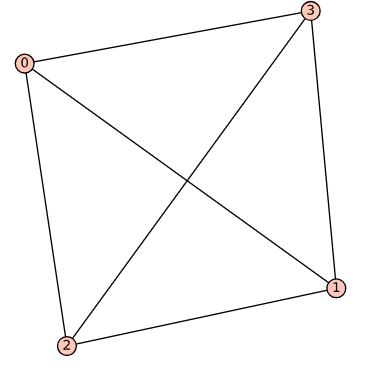
\includegraphics[width=0.6\textwidth]{example.JPG}
\caption{A graph with 4 vertices and 6 edges}
\end{figure}
\begin{newpage}
\end{newpage}

In our next example [Figure 1.2], we have five vertices, representing five persons, Bob, William, James, Chris and Ajur. The edges in the graph represent friendship. Chris is friends with William, James and Ajur. Bob is friends with William and James. This is depicted as a graph in Figure 1.2. It has 5 vertices and 5 edges.
\begin{figure}
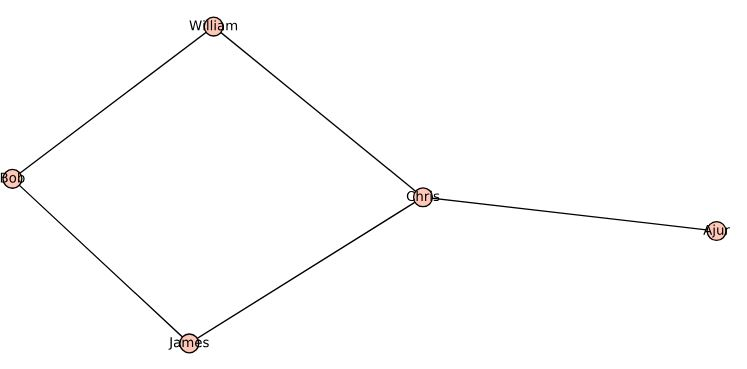
\includegraphics[width=0.9\textwidth]{example2.JPG}
\caption{A friendship graph with 5 vertices and 5 edges}
\end{figure}
\begin{newpage}
\end{newpage}
In our third example [Figure 1.3], we have seven Northeastern states in the United States, namely NY (New York), CT (Connecticut), VT (Vermont), ME (Maine), MA (Massachusetts) RI (Rhode Island) and NH (New Hampshire). The relationship represented is sharing a border with another state. NY borders CT, VT, and MA. CT additionally borders RI and MA. VT borders MA and NH. ME borders NH. MA borders RI and NH. This is depicted in Figure 1.3. It has 7 vertices and 10 edges.

\begin{figure}
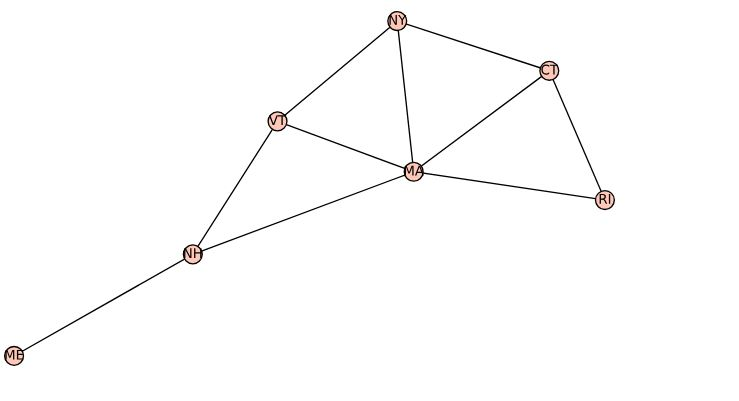
\includegraphics[width=0.9\textwidth]{example3.JPG}
\caption{A graph representing the northeastern United States, with 7 vertices and 10 edges}
\end{figure}
\begin{newpage}
\end{newpage}

If there is an edge between two vertices (like NY and VT in Figure 1.3), we say that these two vertices are \textbf{adjacent}. For instance, NY is adjacent to VT and VT is adjacent to NY.

%\chapter{Introduction}
   

\chapter{Trip to the Cemetery}
It was a Halloween, a cold and dreary evening. Ajur was interested in visiting the famous cemetery in Royt as any teenager with an adventurous spirit would be. His pet dog Jura, a Labrador, was eager to follow him. As Ajur was examining the headstones and tombs, he lost track of time and it was getting dark. He grew tired and he and Jura sat under a tree and they fell asleep. Suddenly they were awakened by a loud noise. The noise was from Rishnak, a ghost who lived in the cemetery. Rishnak had died a few years ago; he used to teach mathematics and graph theory for talented high school students in the area. When Rishnak spotted Ajur in that cemetery, he thought to himself, ``here is an unusual teenager." Perhaps he could test whether this youngster  was proficient in mathematics. If he was indeed proficient, Rishnak could reward him with his magical powers. When Rishnak appeared in front of Ajur, Jura started barking.  

Rishnak was afraid he would intimidate Ajur by being brusque. Jura was barking with loudly. So Rishnak started talking in a soft voice. He gently asked what grade Ajur was in. Ajur replied that he was in middle school and studying in 8th grade. Rishank proceeded to ask the boy what subjects he liked most in school. Ajur proudly added that he was very good in mathematics. Rishnak smiled to himself. He told the boy that he had been cursed to live as ghost and his curse would be lifted if he could reward some youngsters who could answer all his questions. Ajur was intrigued by Rishnak's offer and he jumped at the possibility of rewards, and the opportunity to help lift the curse on a Rishnak, a ghost and tell his friends about his adventure.

\chapter{Degrees}
Rishnak asked Ajur whether he knew about graphs and trees in mathematics. Ajur jumped up and down and proclaimed that he knew all about graph theory. He continued that graphs are often used to  represent relations of a set of objects. He enthusiastically stated that the famous mathematician Euler was the father of graph theory. He was eager to show off his knowledge and described the famous  K\"{o}nigsberg bridge problem.  K\"{o}nigsberg (in modern day Russia) was on the banks of the Pregel river.  There were seven bridges across this river, connecting the two sides of the river and two islands. Ajur drew a graph of this on a piece of paper he was carrying.
\begin{figure}
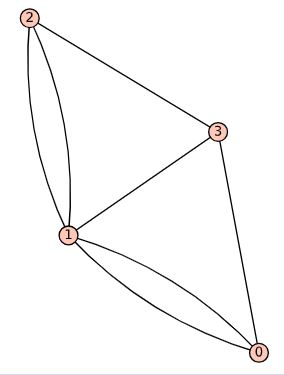
\includegraphics[width=0.6\textwidth]{konigsberg.JPG}
\caption{A Graph representing K\"{o}nigsberg Bridge. Vertices 1 and 3 are islands and 0 and 2 are the two riverbanks.}\label{kon}
\end{figure}

He continued that the problem was to start from the vertex labeled 0 and go through all bridges once and only once and return to the starting vertex 0. Ajur could not contain his enthusiasm and asked Rishnak how to do it. Rishnak gently reminded Ajur that he was the one asking questions and Ajur just had to respond with correct responses. Ajur nodded his head enthusiastically.

 Since this was the first time, Rishnak told Ajur that he was going to ask Ajur a series of questions and observe whether his curses could be lifted.
 
 Rishnak then asked Ajur, ``in a class of 33 students, what is the maximum and minimum number of friends a student can have?"\footnote{Being friend is a mutual relation, i.e. if A is a friend of B, then B is a friend of A. A student cannot be a friend to herself!}
 
 Ajur nonchalantly replied that the maximum number is 32 and the minimum number is 0.
 
 Rishnak then asked Ajur ``will there be a student in a class having 32 friends and a student having 0 friends?"
 
 Ajur smiled to himself that Rishnak seems like a clever ghost; Ajur replied, ``how is that possible --- if a student has 32 friends, so she is friends with everyone else, then everyone else has at least one friend. 
 So there cannot be a 
 student with 0 friends. Similarly if there is a student with 0 friends, there are only 32 students remaining and another student can have at most 31 friends."
 
 Rishnak was pleased to have found someone who seemed to have the ability to help him and the questioning continued. ``Can all the 33 students have a distinct number of friends?"
 
 Ajur responded immediately saying it is not possible because there are 33 distinct students, and the distinct number of friends the class can have is $\{0,1,2,\cdots,32\}$. There are 33 numbers in this, but alas it contains both students with 32 friends and with 0 friends. Ajur just had told Rishnak that it is not possible to have a student with 32 friends and another student with 0 friends.
 
 Rishnak asked Ajur, ``can there be just two students having the same number of friends, with the others all having distinct numbers of friends?" Rishnak further added that all of the students have at least one friend.
 
Ajur wanted to reason it out. He knew that the maximum number can only be 32, and the minimum has to be 1, so there are 32 distinct numbers. But there are 33 students. So by the pigeon hole principle --- if there are more pigeons than boxes, then one box contains at least two pigeons --- there have to be two students with the same number of friends.  He then reasoned about what the numbers could be. He matched 32 with 1: that is, the student having one friend has to be a friend of a student with 32 friends. Then he matched 2 with 31: the student with 2 friends has to be a friend of a student with 32 friends and a student with 31 friends. Continuing this argument, he matched 3 with 30, 4 with 29, $\cdots$, 15 with 18 and 16 with 17. We have an even number of students accounted for but an odd number of total students. That means there are two students having the same number of friends.

Rishnak posed the next question: He asked 5 students in a class of 6 students how many friends each of them have and they all gave distinct numbers greater than 0. How many friends does the student who was not asked have?

Ajur thought about this. If all the five students had given distinct numbers and they were greater than 0, they had to be $\{1,2,3,4,5\}$. Let the students be A(pu), B(art), C(arla), D(uma), E(rnie) having 5, 4, 3, 2 and 1 friends respectively. Let F(orme) be the sixth student. A is friends with B, C, D, E and F. B is friends with C, D and F. B is already friends with A and E has only one friend, namely A. Now C is friends with F. C is already friends with A and B, and D and E have their friends quota counted already. 
Now it is easy to see that F(orme) has exactly 3 friends, namely A, B and C.

Ajur drew the following graph as in Figure 3.2

\begin{figure}
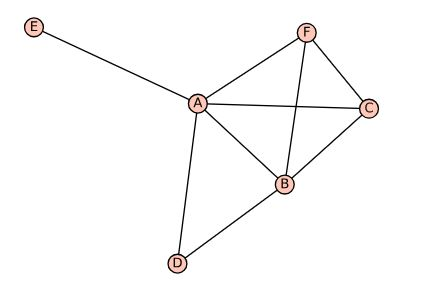
\includegraphics[width=0.6\textwidth]{graphstory1-1.JPG}
\caption{A Graph with 6 students and 5 students having 5, 4, 3, 2 and 1 friends}
\end{figure}

Rishnak was impressed, but wanted to test Ajur further. He asked whether there can an be odd number of students having odd number of friends. Ajur said that it is impossible as the sum of all numbers of friends across all students has to be even. He reasoned that if A is a friend of B, then this friendship is counted twice. Hence the sum of all friends of students is even. We know that the students having an even number of friends will contribute an even number of friendships. This in turn implies that the number of students having an odd number of friends has to be even.


Rishnak started asking, ``can you draw a graph of a class with 5 students respectively having 1, 2, 2, 2 and 1 friends?"

Ajur whipped up the graph drawn in Figure 3.3. 

\begin{figure}
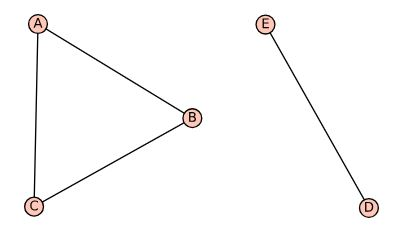
\includegraphics[width=0.6\textwidth]{graphstory1-2.JPG}
\caption{A Graph with 5 students having 2, 2, 2, 1 and 1 friends}
\end{figure}

Rishnak asked whether one can draw another graph having the given friends list.\footnote{Hakimi has given a method of constructing a graph with a given degree sequence}

Ajur took no time to respond and drew another graph as in Figure 3.4.

\begin{figure}
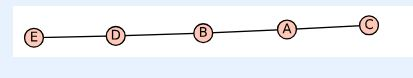
\includegraphics[width=0.6\textwidth]{graphstory1-3.JPG}
\caption{Another Graph with 5 students having 2, 2, 2, 1 and 1 friends}
\end{figure}

Jura was waking up and wanted to play with Ajur. Rishnak was happy to see the answers that Ajur gave. He saw a ray of hope that his curse could be lifted. 

Rishnak told Ajur to come back the next night, and he disappeared in a cold mist.

%\chapter{Puzzle 2}
\chapter{Rooted Trees and Trees}

Rishnak found Ajur and his dog Jura walking along a row of graves. Ajur was reading the inscriptions on the tombstones. Each headstone had the names of the family (parents, wife, husband) and the dates of birth and of death. Ajur did not know so many relatives could be buried in such a small area. He then thought of how different cultures honor their departed ones \footnote{He remembered seeing the movie Coco in 2017 about how people in Mexico remember their departed ones. He had also heard how Hindus in India go to the city of Banaras/Varanasi to perform rituals to thank and honor their deceased forefathers.} 
Ajur remembered the definition of a tree and a rooted tree. He was talking to Jura, saying that a rooted tree in graph theory/mathematics looks like a normal tree with a distinguished vertex. A rooted tree in real life has a root at the bottom whereas a rooted tree in graph theory is drawn with a root at the top. Both of them convey the same information.

``Here are two drawings of the same information." Ajur further explained that each vertex in a rooted tree has just one parent vertex (except the root vertex which has no parent). A rooted tree can also be thought of as a graph with a collection of vertices and edges. There are some restrictions. But that will become clearer, as the story proceeds.


\begin{figure}
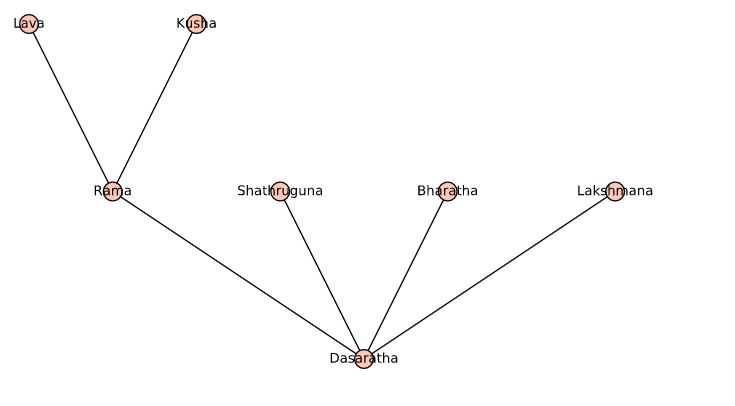
\includegraphics[width=\textwidth]{tree1.JPG}
\caption{A Tree drawn with a root at the bottom}
\end{figure}

\begin{figure}
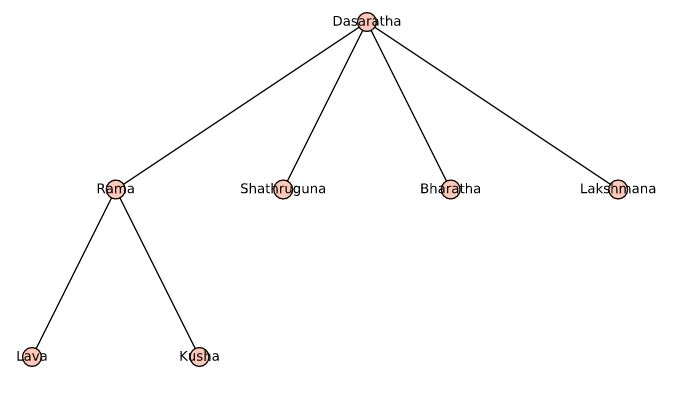
\includegraphics[width=\textwidth]{tree2.JPG}
\caption{Same Tree drawn with a root at the top}
\end{figure}

Rishnak caught up with Ajur and Jura as he had been following them quietly. Rishnak asked Ajur: ``how many edges does a rooted tree with 7 vertices have?" Ajur reasoned that since each vertex other than the root has exactly one parent vertex and there are no other edges, then number of edges will be 6. Rishnak then asked how many edges a rooted tree with 1000 vertices has. Ajur shot back with his answer 999. Impressed, but not unduly, Rishnak asked how many edges there are in a rooted tree with $n$ vertices. Nonchalantly, Ajur replied it is $n-1$ by the same argument (each of the $n-1$ vertices have just one edge connected to its parent).  

For each vertex other than a root vertex, there is a parent vertex and zero or more child vertices.  The descendants of a vertex are all its children, grandchildren, great grandchildren vertices etc. Analogously, for each vertex the ancestors of that vertex are its parent, grandparent, great grandparent vertices etc. 
A vertex with no child vertices is known as a leaf vertex. Rishnak asked Ajur ``what is the largest number of leaf vertices a tree with 6 vertices can have?" Ajur immediately responded that the number is 5, and he drew a rooted tree as in Figure \ref{t1}.

\begin{figure}
\begin{center}
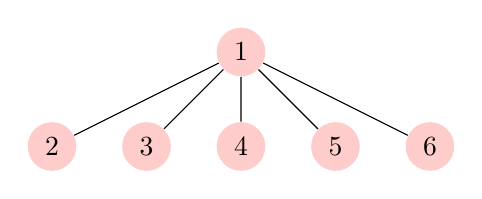
\begin{tikzpicture}
  [scale=.6,auto=left,every node/.style={circle,fill=red!20}]
  \node (n6) at (5,5) {1};
  \node (n4) at (1,3)  {2};
  \node (n5) at (3,3)  {3};
  \node (n1) at (5,3) {4};
  \node (n2) at (7,3)  {5};
  \node (n3) at (9,3)  {6};

  \foreach \from/\to in {n6/n1,n6/n2,n6/n3,n6/n4,n6/n5}
    \draw (\from) -- (\to);

\end{tikzpicture}

\caption{A Tree with 6 vertices and 5 leaf vertices. The vertex labeled 1 is the root vertex}\label{t1}
\end{center}
\end{figure}

Rishnak asked, ``what is the smallest number of leaf vertices a tree with 6 vertices can have?" Ajur knew this answer too. So he drew a rooted tree as in Figure~\ref{t2}.

\begin{figure}
\begin{center}
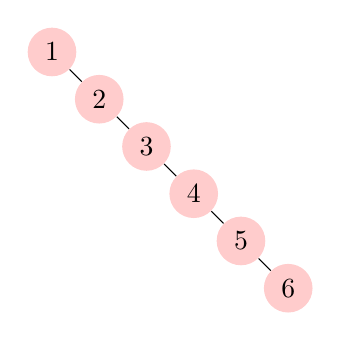
\begin{tikzpicture}
  [scale=.6,auto=left,every node/.style={circle,fill=red!20}]
  \node (n6) at (3,7) {1};
  \node (n4) at (4,6)  {2};
  \node (n5) at (5,5)  {3};
  \node (n1) at (6,4) {4};
  \node (n2) at (7,3)  {5};
  \node (n3) at (8,2)  {6};

  \foreach \from/\to in {n6/n4,n4/n5,n5/n1,n1/n2,n2/n3}
    \draw (\from) -- (\to);

\end{tikzpicture}

\caption{A Tree with 6 vertices and one leaf vertex labeled 6. The vertex labeled 1 is the root vertex.}\label{t2}
\end{center}
\end{figure}

Rishnak said ``We get a lot of lightning and thunderstorms here, especially during summer months. Lightning affects tall objects, especially objects that conduct electricity in an open area\footnote{Benjamin Franklin had demonstrated the electrical nature of lightning}. Lightning conductors are usually at the top of the buildings and have less resistance than the building, and hence lightning passes through the conductor." Rishnak drew a rooted tree with 3 vertices as shown in Figure~\ref{t3}.

\begin{figure}
\begin{center}

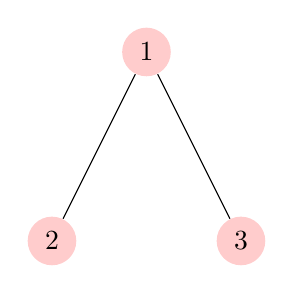
\begin{tikzpicture}
  [scale=.6,auto=left,every node/.style={circle,fill=red!20}]
  \node (n1) at (3,7) {1};
  \node (n2) at (1,3)  {2};
  \node (n3) at (5,3)  {3};


  \foreach \from/\to in {n1/n2,n1/n3}
    \draw (\from) -- (\to);

\end{tikzpicture}

\caption{A resistance  Tree with 3 vertices and two leaf vertices at the ground. }\label{t3}
\end{center}
\end{figure}


Rishnak said that the each edge has a resistance of 1 ohm, and vertices labeled 2 and 3 are grounded. What is the effective resistance of the resistance tree in Figure~\ref{t3}? Ajur remembered his physics and he realized two resistances are in parallel. So he immediately replied that the effective resistance is $\frac{1}{2}$ ohms. (Intuitively, there are two paths the current can take and hence the resistance splits evenly between the 2 paths).

Rishnak asked the same question, effective resistance, for the following rooted tree shown in Figure \ref{t4}.
\begin{figure}
\begin{center}

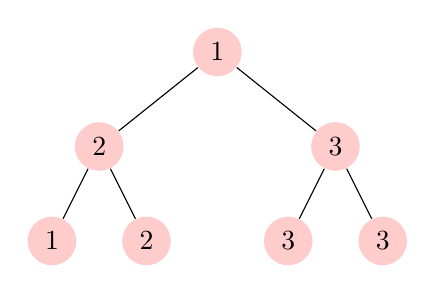
\begin{tikzpicture}
  [scale=.6,auto=left,every node/.style={circle,fill=red!20}]
  \node (n1) at (5.5,7) {1};
  \node (n2) at (3,5)  {2};
  \node (n3) at (8,5)  {3};
  \node (n4) at (2,3) {1};
  \node (n5) at (4,3)  {2};
  \node (n6) at (7,3)  {3};
  \node (n7) at (9,3)  {3};

  \foreach \from/\to in {n1/n2,n1/n3,n2/n4,n2/n5,n3/n6,n3/n7}
    \draw (\from) -- (\to);

\end{tikzpicture}

\caption{A resistance  Tree with 7 vertices and four leaf vertices at the ground. }\label{t4}
\end{center}
\end{figure}

Ajur said that he had computed the effective resistances for trees rooted at vertex labeled 2 and 3 to be $\frac{1}{2}$. There are two parallel paths with equal resistance of $1+\frac{1}{2}$ (There is a series connection from root vertex 1 and vertices labeled 2 and 3 respectively). Hence the effective resistance is $\frac{3}{4}$ ohms. Ajur further said that there is a pattern here. For the resistance tree with 15 vertices (adding one more level or increasing the height), the effective resistance will be $\frac{7}{8}$. Rishnak then asked what happens if the tree is of infinite height! (A really tall lightning conductor.) Ajur was perplexed - But then he reasoned that this could be formulated as a recurrence relation. Let R be the effective resistance of this infinite tree. The root has two children, each of which will have a resistance of R ohms. The root vertex is connected to the child vertex with a resistance of 1 ohm. Hence he wrote an equation $$R= \frac{R+1}{2}$$ Simplifying this, he got the resistance of 1 ohm. A really tall lightning conductor (a tree of infinite height) with a very low resistance - hence an excellent lightning conductor.\footnote{Because of a large number of joints, this solution may not be a practical one!} Rishnak responded that there is another way of getting the same result. From an earlier example, you can generalize the resistance to be $\frac{2^h-1}{2^h}$ , $h$ being height (longest among path lengths from the root vertex to all leaf vertices) of the rooted tree. This can be further simplified to be $1-\frac{1}{2^h}$. As $h$ goes to infinity the term $\frac{1}{2^h}$ goes to 0 and hence the resistance is 1. Ajur learned an important lesson that there are multiple ways of getting a solution and each one may provide a new insight. Ajur asked Rishnak: ``can you construct an infinite height tree (with edge resistances being one ohm) so that the effective resistance is $\frac{1}{2}$, $\frac{1}{3}$, $\frac{1}{4}$ or more generally any fraction $\leq$~1?" Rishnak replied to Ajur that he was the one who could ask questions and not Ajur.\footnote{Of course Rishnak knew the answer and suggests others to think every vertex having more than 2 child vertices!}

A tree is like a rooted tree but with no root vertex. A tree can be drawn in any manner. The degree of a vertex is the number of edges incident on that vertex. The leaf (pendant) vertex has a degree of 1. So in Figure~\ref{t2} both vertices labeled 1 and 6 are leaf/pendant vertices and all other vertices have degree 2. 

Rishnak told Ajur that one important property of a tree is that there are no cycles in it. Ajur could easily understand it from a genealogy perspective - a person cannot be an ancestor as well as a descendant of himself/herself.  Ajur added that there is only one path between any two vertices in a tree (Of course, Ajur assumed that the edges are undirected --- which Rishnak knew). Rishnak asked ``how did you infer that there is a unique path between two vertices in a tree?" Ajur promptly replied that if there are two paths between any two vertices, there will be a cycle (which cannot exist in a tree). Since there is an unique path between two vertices, one can compute the distance between two vertices as the number of edges in that path. Ajur provided clarifications with examples.  As an example in Figure~\ref{t1}, the distance between the vertex labeled 1 and any other vertex is 1. The distance between the vertex labeled 2 and the vertex labeled 6 is 2. In Figure~\ref{t2}, the distance between the vertex labeled 1 and the vertex labeled 6 is 5 and the distance between the vertex labeled 2 and the vertex labeled 4 is 2.
%(Dad: you could also add the fact that every finite tree has a center of mass! it's in this vein, and not especially well known (Boris hadn't realized it!))
\chapter{Subgraphs}
Rishnak found Ajur sleeping with his dog Jura near the cemetery and saw a headstone nearby with the name Schossow. Rishnak recognized the name  from Instant Insanity Puzzle{\footnote{It is also known as Katzenjammer, (Great) Tantalizer, Face-4, Cube-4, Bognar Balls, Taktikolor, Frantic, Diabolical, Damblocks,
Symington's Puzzle. A patent was awarded to  Schossow in 1990}}. Just as Rishnak was thinking it would be an interesting topic to discuss with Ajur, Jura the dog, eager to explore, nudged Ajur. Before long, Ajur and Jura were strolling along a path where Rishnak startled Ajur (as ghosts tend to do). 

Rishnak asked Ajur what he knew about subgraphs. Ajur said that he was familiar with subsets. Since a graph has both a vertex set and edge set, he can deduce what a subgraph is. If a graph $G=(V,E)$ with a vertex set $V$ and an edge set $E$, then take any subset $X$ of $V$ and consider all the edges in E, which has both its end vertices in $X$. Ajur drew this.
\vspace{0.2in}
\\
\noindent
\begin{figure}
\begin{center}
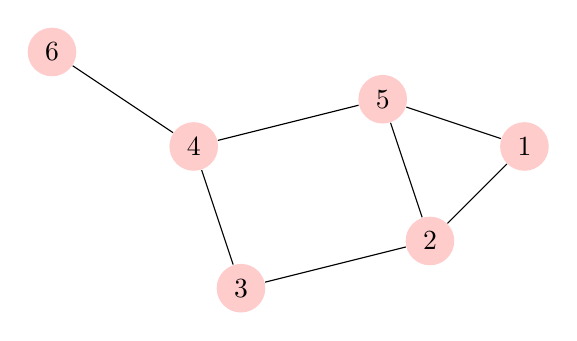
\begin{tikzpicture}
  [scale=.6,auto=left,every node/.style={circle,fill=red!20}]
  \node (n6) at (1,10) {6};
  \node (n4) at (4,8)  {4};
  \node (n5) at (8,9)  {5};
  \node (n1) at (11,8) {1};
  \node (n2) at (9,6)  {2};
  \node (n3) at (5,5)  {3};

  \foreach \from/\to in {n6/n4,n4/n5,n5/n1,n1/n2,n2/n5,n2/n3,n3/n4}
    \draw (\from) -- (\to);

\end{tikzpicture}
\caption{ Example Graph with 6 vertices and 7 edges}\label{3g}
\end{center}
\end{figure}
\\
\noindent
If one took a vertex subset $\{1,2,3,5\}$ of Figure \ref{3g} the subgraph could be as in Figure \ref{3g1}.
\begin{figure}
\begin{center}
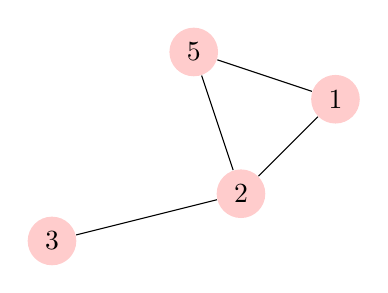
\begin{tikzpicture}
  [scale=.6,auto=left,every node/.style={circle,fill=red!20}]
  %\node (n6) at (1,10) {6};
  %\node (n4) at (4,8)  {4};
  \node (n5) at (8,9)  {5};
  \node (n1) at (11,8) {1};
  \node (n2) at (9,6)  {2};
  \node (n3) at (5,5)  {3};

  \foreach \from/\to in {n5/n1,n1/n2,n2/n5,n2/n3}
    \draw (\from) -- (\to);
\end{tikzpicture}
\caption{Induced Subraph of Figure \ref{3g} Vertices 1,2,3 and 5 are chosen and all the edges between these vertices which are present in the original graph have to be in this subgraph}\label{3g1}
\end{center}
\end{figure}
\\
\noindent
Rishnak laughed and said that the subgraph Ajur drew was called an \textit {induced subgraph} --- that is, all the edges are included in the vertex subset. You have the flexibility of choosing only a subset of these edges. But there is one extra condition: for each edge in the chosen subset of edges, the end vertices should be in the chosen vertex subset. 
\\
\begin{figure}
\begin{center}
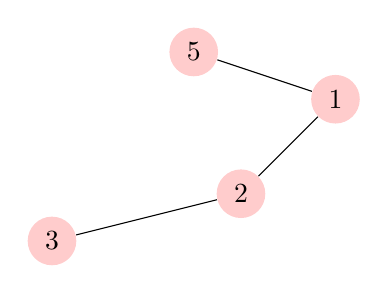
\begin{tikzpicture}
  [scale=.6,auto=left,every node/.style={circle,fill=red!20}]
  %\node (n6) at (1,10) {6};
  %\node (n4) at (4,8)  {4};
  \node (n5) at (8,9)  {5};
  \node (n1) at (11,8) {1};
  \node (n2) at (9,6)  {2};
  \node (n3) at (5,5)  {3};

  \foreach \from/\to in {n5/n1,n1/n2,n2/n3}
    \draw (\from) -- (\to);

\end{tikzpicture}
\caption{A subgraph of Figure \ref{3g}}\label{3g2}
\end{center}
\end{figure}
\\
\noindent
Rishnak illustrated this with the following subgraph example as shown in Figure \ref{3g2}. A subgraph with no vertices and no edges is also an induced subgraph (and subgraph) of any graph.


%Rishnak said that in a graph having $n$ vertices where the vertices are labeled (have a number/name associated with them), then there are at least $2^n$ subgraphs and exactly $2^n$ induced subgraphs.  There are ${n \choose i}$ ways of choosing $i$ vertices from a given set of $n$ vertices. Once the vertices are chosen, the edges are fixed for an induced subgraph. Since $i$ can vary from 0 to $n$, we get $2^n$ induced subgraphs. Since every induced subgraph is a subgraph (and not every subgraph is not an induced subgraph), we have at least $2^n$ subgraphs.  

A walk from a vertex $i$ to a vertex $j$ is an alternating sequence of vertices and edges. Every edge in that walk is incident between vertices preceding and succeeding that edge. For example in Figure \ref{3g},
a walk from vertex 6 to vertex 1 could be 6 (6,4), 4, (4,3), 3, (3,2), 2, (2,1) and 1. The edges are represented as a vertex pair. If those edges are labelled with a name, that label could be used instead. Another walk in Figure \ref{3g} from vertex 6 to vertex 1 could be 6, (6,4), 4, (4,5), 5 (5,1), 1.  The only other condition that the walk has (besides an edge being incident on a preceding and a succeeding vertex) is that all the edges have to be distinct. However the vertices in a walk can be repeated. 
Here is another example Figure \ref{3g3}. A walk from vertex 1 and vertex 8 could be 1, (1,2), 2, (2,4), 4, (4,6), 6, (6,8) and 8. (8,2), 2, (2,3), 3, (3,4), 4, (4,5), 5, (5,6), 6, (6,7), 7, (7,8) and 8. Ajur was naturally getting bored. He interjected that in your walk you have visited all the edges in the graph (shown in Figure \ref{3g3}). Ajur further added that this was similar to the K\"{o}nigsberg Bridge Problem (Figure \ref{kon} mentioned earlier in Chapter 3!).  
\begin{figure}
\begin{center}
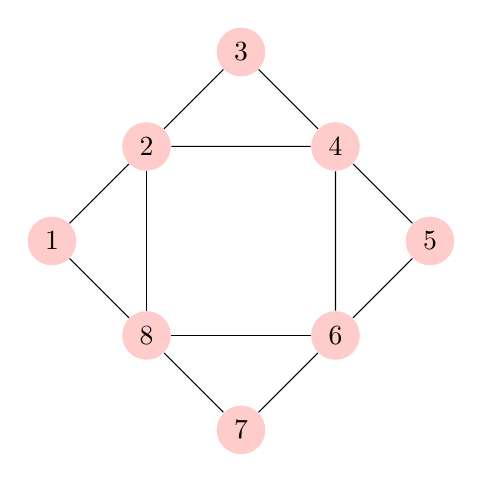
\begin{tikzpicture}
  [scale=.6,auto=left,every node/.style={circle,fill=red!20}]
  \node (n1) at (1,7) {1};
  \node (n2) at (3,9)  {2};
  \node (n3) at (5,11)  {3};
  \node (n4) at (7,9) {4};
  \node (n5) at (9,7)  {5};
  \node (n6) at (7,5)  {6};
  \node (n7) at (5,3)  {7};
  \node (n8) at (3,5)  {8};

  \foreach \from/\to in {n1/n2,n1/n8,n2/n3,n2/n4,n2/n8,n3/n4,n4/n5,n4/n6,n5/n6,n6/n7,n6/n8,n7/n8}
    \draw (\from) -- (\to);

\end{tikzpicture}
\caption{ Example Graph with 8 vertices and 12 edges}\label{3g3}
\end{center}
\end{figure}
\\

If the starting and ending vertices in a walk are the same, it is known as a closed walk. If all the edges in a closed walk are distinct, then it is known as a cycle. 
Ajur had heard of this from his friends.
Rishnak asked Ajur to list two cycles from Figure \ref{3g3}. Ajur had no trouble at all, in listing two cycles as (1,(1,2),2,(2,8),8,(8,1),1) and (2,(2,4),4,(4,6),6,(6,8),8,(8,2)2). Often the edges are omitted, and the cycles are written as (1,2,8,1) and (2,4,6,8,2).  Of course, a cycle and a walk are examples of subgraphs with some added conditions. These added conditions make the study of subgraphs very interesting. If in a cycle, all the vertices of the original graph are present, then that cycle is known as a Hamiltonian Cycle. For example in Figure \ref{3g3} the cycle (1,2,3,4,5,6,7,8,1) is a Hamiltonian Cycle of Figure \ref{3g4}. If all the edges in a walk are distinct then it is known as a path. Ajur gave the following examples for a path in Figure \ref{3g3} as (1,(1,2),2,(2,3),3) or simply as (1,2,3), Figure \ref{3g5}. If there is a path between every pair of vertices in a subgraph, then the subgraph is said to be connected. If a subgraph contains no cycles and is connected, the subgraph is a tree. If such a tree contains all vertices then it is known as spanning tree, Figure \ref{3g6}.  A subgraph in which the degree of every vertex is 1 is called a matching. An example of a subgraph (which is a matching for Figure \ref{3g3}) is in Figure \ref{3g7}. If the subgraph contains all vertices and the degree of every vertex is one, then it is called as Perfect matching. An example of a subgraph that is a perfect matching for Figure~\ref{3g3} is in Figure \ref{3g8}. Rishnak asked Ajur how many perfect matchings there are in Figure \ref{3g3}. Ajur thought a bit. He saw vertices 1, 3, 5 and 7 hae degree 2. Hence one of those incident on 1, 3, 5 and 7 have to be selected. Hence he replied that there are exactly two perfect matchings in Figure \ref{3g3}. 
\\
\begin{figure}
\begin{center}
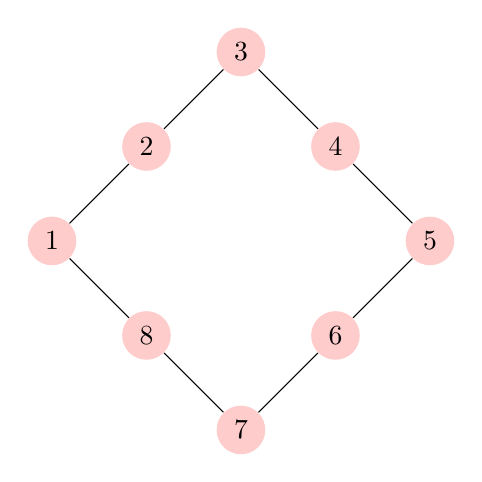
\begin{tikzpicture}
  [scale=.6,auto=left,every node/.style={circle,fill=red!20}]
  \node (n1) at (1,7) {1};
  \node (n2) at (3,9)  {2};
  \node (n3) at (5,11)  {3};
  \node (n4) at (7,9) {4};
  \node (n5) at (9,7)  {5};
  \node (n6) at (7,5)  {6};
  \node (n7) at (5,3)  {7};
  \node (n8) at (3,5)  {8};

  \foreach \from/\to in {n1/n2,n1/n8,n2/n3,n3/n4,n4/n5,n5/n6,n6/n7,n7/n8}
    \draw (\from) -- (\to);

\end{tikzpicture}
\caption{ A subgraph which is a Hamiltonian Cycle}\label{3g4}
\end{center}
\end{figure}

\begin{figure}
\begin{center}
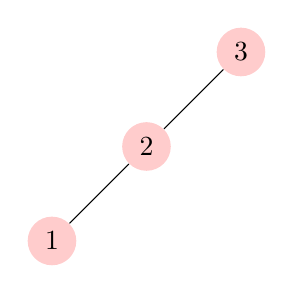
\begin{tikzpicture}
  [scale=.6,auto=left,every node/.style={circle,fill=red!20}]
  \node (n1) at (1,7) {1};
  \node (n2) at (3,9)  {2};
  \node (n3) at (5,11)  {3};


  \foreach \from/\to in {n1/n2,n2/n3}
    \draw (\from) -- (\to);

\end{tikzpicture}
\caption{ A subgraph which is a tree}\label{3g5}
\end{center}
\end{figure}

\begin{figure}
\begin{center}
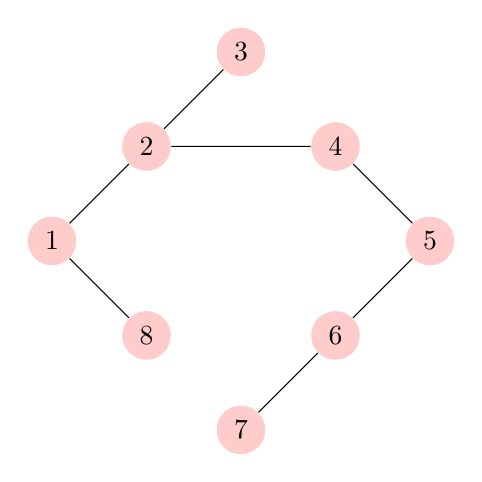
\begin{tikzpicture}
  [scale=.6,auto=left,every node/.style={circle,fill=red!20}]
  \node (n1) at (1,7) {1};
  \node (n2) at (3,9)  {2};
  \node (n3) at (5,11)  {3};
  \node (n4) at (7,9) {4};
  \node (n5) at (9,7)  {5};
  \node (n6) at (7,5)  {6};
  \node (n7) at (5,3)  {7};
  \node (n8) at (3,5)  {8};

  \foreach \from/\to in {n1/n2,n1/n8,n2/n3,n2/n4,n4/n5,n5/n6,n6/n7}
    \draw (\from) -- (\to);

\end{tikzpicture}
\caption{ A subgraph which is a spanning tree}\label{3g6}
\end{center}
\end{figure}

\begin{figure}
\begin{center}
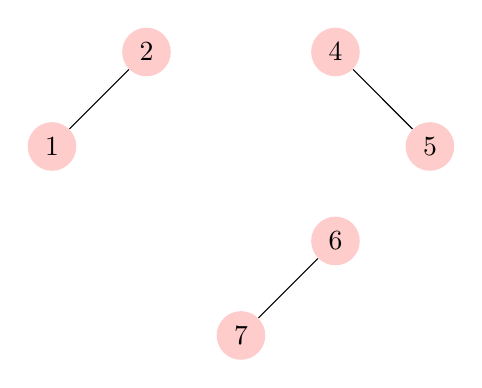
\begin{tikzpicture}
  [scale=.6,auto=left,every node/.style={circle,fill=red!20}]
  \node (n1) at (1,7) {1};
  \node (n2) at (3,9)  {2};
  %\node (n3) at (5,11)  {3};
  \node (n4) at (7,9) {4};
  \node (n5) at (9,7)  {5};
  \node (n6) at (7,5)  {6};
  \node (n7) at (5,3)  {7};
  %\node (n8) at (3,5)  {8};

  \foreach \from/\to in {n1/n2,n4/n5,n6/n7}
    \draw (\from) -- (\to);

\end{tikzpicture}
\caption{ A subgraph which is a matching}\label{3g7}
\end{center}
\end{figure}

\begin{figure}
\begin{center}
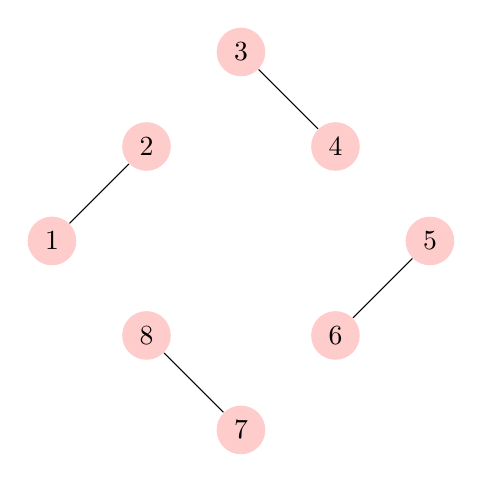
\begin{tikzpicture}
  [scale=.6,auto=left,every node/.style={circle,fill=red!20}]
  \node (n1) at (1,7) {1};
  \node (n2) at (3,9)  {2};
  \node (n3) at (5,11)  {3};
  \node (n4) at (7,9) {4};
  \node (n5) at (9,7)  {5};
  \node (n6) at (7,5)  {6};
  \node (n7) at (5,3)  {7};
  \node (n8) at (3,5)  {8};

  \foreach \from/\to in {n1/n2,n3/n4,n5/n6,n7/n8}
    \draw (\from) -- (\to);

\end{tikzpicture}
\caption{ A subgraph which is a perfect matching}\label{3g8}
\end{center}
\end{figure}

\vspace{3in}
A graph is connected if there is a path between every pair of vertices in that graph. Otherwise the graph is disconnected,  Here is an example of a connected graph, Figure \ref{3g9}. Here is an example of a graph that is not connected, Figure \ref{3g10}
\begin{figure}
\begin{center}
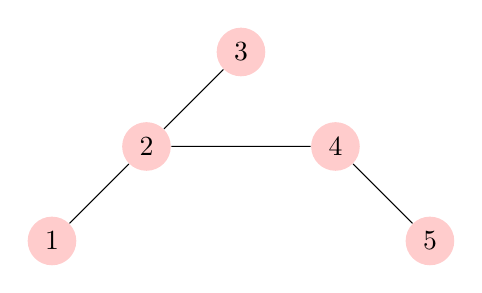
\begin{tikzpicture}
  [scale=.6,auto=left,every node/.style={circle,fill=red!20}]
  \node (n1) at (1,7) {1};
  \node (n2) at (3,9)  {2};
  \node (n3) at (5,11)  {3};
  \node (n4) at (7,9) {4};
  \node (n5) at (9,7)  {5};
\foreach \from/\to in {n1/n2,n2/n3,n2/n4,n4/n5}
    \draw (\from) -- (\to);

\end{tikzpicture}
\caption{ A connected graph}\label{3g9}
\end{center}
\end{figure}

\begin{figure}
\begin{center}
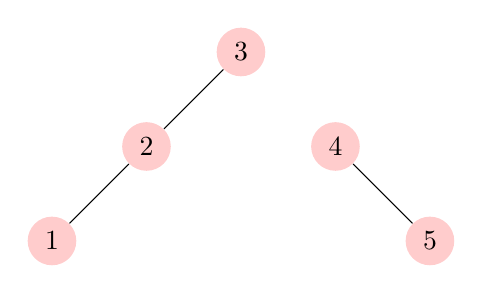
\begin{tikzpicture}
  [scale=.6,auto=left,every node/.style={circle,fill=red!20}]
  \node (n1) at (1,7) {1};
  \node (n2) at (3,9)  {2};
  \node (n3) at (5,11)  {3};
  \node (n4) at (7,9) {4};
  \node (n5) at (9,7)  {5};
\foreach \from/\to in {n1/n2,n2/n3,n4/n5}
    \draw (\from) -- (\to);

\end{tikzpicture}
\caption{ A graph that is not connected}\label{3g10}
\end{center}
\end{figure}
\vspace{3in}

\textbf{Question for the third day:} Rishnak asked Ajur to list the cycles in the following graph Figure \ref{day3g1} 

\begin{figure}
\begin{center}
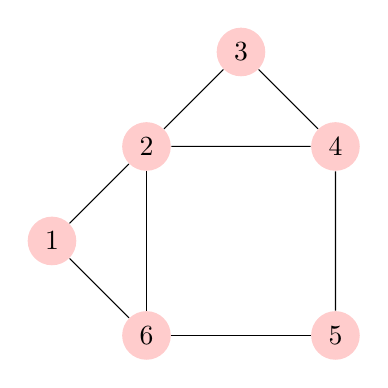
\begin{tikzpicture}
  [scale=.6,auto=left,every node/.style={circle,fill=red!20}]
  \node (n1) at (1,7) {1};
  \node (n2) at (3,9)  {2};
  \node (n3) at (5,11)  {3};
  \node (n4) at (7,9) {4};
  \node (n5) at (7,5)  {5};
  \node (n6) at (3,5)  {6};

  \foreach \from/\to in {n1/n2,n1/n6,n2/n3,n2/n4,n2/n6,n3/n4,n4/n5,n5/n6}
    \draw (\from) -- (\to);

\end{tikzpicture}
\caption{ How many Cycles are there in this Graph?}\label{day3g1}
\end{center}
\end{figure}

\textbf{Answer:} Ajur listed the 6 cycles as follows:
\begin{enumerate}
    \item Cycle of length 3 (two namely  (1,2,6), (2,3,4)
    \item Cycle of length 4 (one namely) (2,4,5,6)
    \item Cycle of length 5 (two namely) (2,3,4,5,6), (1,2,4,5,6)
    \item Cycle of length 6 (one namely) (1,2,3,4,5,6)
\end{enumerate}
Rishnak  was pleased and noticed that Ajur was getting restless, and so was Jura, and so they called it a day.
\chapter{Euler Paths/Cycles}

Ajur was tired after listening to a lot of definitions and examples. He complained to Jura that looked too much like a Math class and he preferred fun Math problems instead. As Ajur was mentioning, Rishnak was overhearing this conversation. Rishnak too felt that the pprvious day's conversation was very cut and dry. His ghost friends were accusing of making the beautiful subject of Graph Theory dull and monotnous.


An Euler walk of a connected graph is a walk that includes every edge exactly once. If the starting vertex and the ending vertex are the same then it is called a closed Euler walk. Of course the name Euler comes from 
Rishnak decided to take on the oldest problem on Graph Theory Euler walk and closed Euler walk. Rishnak caught up with Ajur and Jura walking along a desolate road. Rishnak asked Ajur in the Figure \ref{4g1} whether there is a walk starting from vertex 2 to vertex 4 passing all the edges exactly once [This is what is known as an Eulerian walk]. Ajur saw there is a cycle (2,3,4,1,2). After this cycle, there is just one edge (2,4) left. Hence Ajur constructed an Eulerian walk by combining the two as (2,(2,3),3,(3,4),4,(4,1),1,(1,2),2,(2,4),4) or written simply as (2,3,4,1,2,3) by omitting the edges. Ajur illustrated this Figure \ref{4g15} Ajur further added that there is no closed Eulerian walk as that would imply that the edges have to be split into cycles (with no edges in common among the cycles). This will mean that the degrees of every vertex has to be even. Rishnak was much impressed with Ajur's reasoning. 


\begin{figure}
\begin{center}
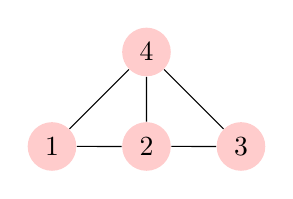
\begin{tikzpicture}
  [scale=.6,auto=left,every node/.style={circle,fill=red!20}]
  \node (n1) at (1,7) {1};
  \node (n2) at (3,7)  {2};
  \node (n3) at (5,7)  {3};
  \node (n4) at (3,9)  {4};

  \foreach \from/\to in {n1/n2,n2/n3,n2/n4,n1/n4,n3/n4}
    \draw (\from) -- (\to);

\end{tikzpicture}
\caption{ Example Graph with 4 vertices and 5 edges}\label{4g1}
\end{center}
\end{figure}

\begin{figure}
\begin{center}
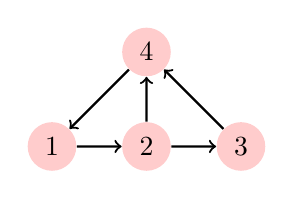
\begin{tikzpicture}
  [scale=.6,auto=left,every node/.style={circle,fill=red!20}]
  \node (n1) at (1,7) {1};
  \node (n2) at (3,7)  {2};
  \node (n3) at (5,7)  {3};
  \node (n4) at (3,9)  {4};

\path [->,draw,thick]
(n2) edge  (n3)
(n3) edge   (n4)
(n4) edge   (n1)
(n1) edge   (n2)
(n2) edge  (n4)
;
\end{tikzpicture}
\caption{ Eulerian Path from vertex 2 to vertex 4 2-3-4-1-2-4 of Figure \ref{4g1}}\label{4g15}
\end{center}
\end{figure}
\vspace{2cm}
Rishnak then asked Ajur whether you can start a walk from vertex 1 to vertex 9 and visit all edges once and only once (Eulerian walk from vertex 1 to vertex 9) in connected graph in Figure \ref{4g2}.
Ajur was perplexed. Then he tried to reason - he can break them into cycles. (2,3,7),(7,6,5,4), (3,4,8)  - None of these cycles had any edge in common. So he constructed a 
walk as (1,(1,2),2,(2,3),3,(3,4),4,(4,8),8,(8,3),3,(3,7),7, (7,6),6,(6,5),5,(5,4).4,(4,7),7,(7,2),2,(2,8),8,(8,9),9). Ajur further explained that he obtained this Eulerian walk by essentially by combining these cycles. He illustrated his walk in \ref{4g25}. Ajur responded that there is no closed Eulerian walk in this graph \ref{4g2} as all the vertices are not of even degree. An Eulerian walk startes from a vertex with odd degree and ends at a vertex with odd degree (There has tyo be exactly two vertices .

\begin{figure}
\begin{center}
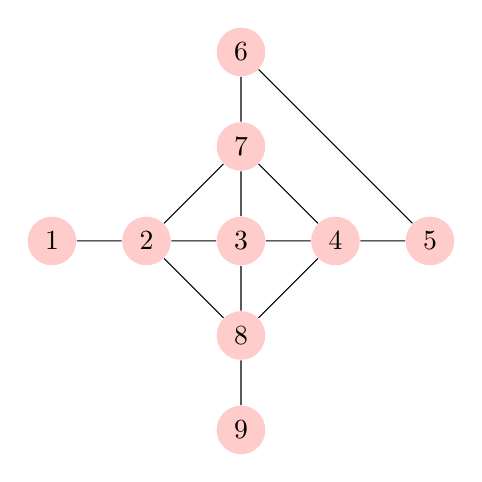
\begin{tikzpicture}
  [scale=.6,auto=left,every node/.style={circle,fill=red!20}]
  \node (n1) at (1,7) {1};
  \node (n2) at (3,7)  {2};
  \node (n3) at (5,7)  {3};
  \node (n4) at (7,7) {4};
  \node (n5) at (9,7)  {5};
  \node (n6) at (5,11)  {6};
   \node (n7) at (5,9) {7};
   \node (n8) at (5,5) {8};
   \node (n9)  at (5,3) {9};
  \foreach \from/\to in {n1/n2,n2/n3,n3/n4,n4/n5,n6/n7,n7/n3,n3/n8,n8/n9,n2/n7,
  n4/n7,n4/n8,n8/n2,n6/n5}
    \draw (\from) -- (\to);

\end{tikzpicture}
\caption{ Example Graph with 9 vertices and 13 edges}\label{4g2}
\end{center}
\end{figure}

\begin{figure}
\begin{center}
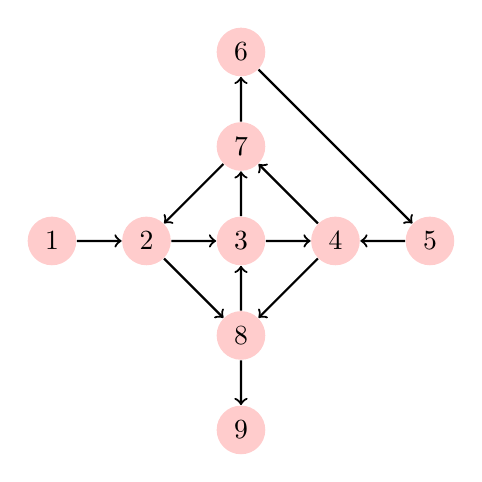
\begin{tikzpicture}
  [scale=.6,auto=left,every node/.style={circle,fill=red!20}]
  \node (n1) at (1,7) {1};
  \node (n2) at (3,7)  {2};
  \node (n3) at (5,7)  {3};
  \node (n4) at (7,7) {4};
  \node (n5) at (9,7)  {5};
  \node (n6) at (5,11)  {6};
   \node (n7) at (5,9) {7};
   \node (n8) at (5,5) {8};
   \node (n9)  at (5,3) {9};
 \path [->,draw,thick] 
  (n1) edge  (n2)
  (n2) edge (n3)
  (n3) edge (n4)
  (n4) edge (n8)
  (n8) edge (n3)
  (n3) edge (n7)
  (n7) edge (n6)
  (n6) edge (n5)
  (n5) edge (n4)
  (n4) edge (n7)
  (n7) edge (n2)
  (n2) edge (n8)
  (n8) edge (n9)
;
\end{tikzpicture}
\caption{ Eulerian Walk from vertex 1 to vertex 9  1-2-3-4-8-3-7-6-5-4-7-2-8-9 of Figure \ref{4g2}}\label{4g25}
\end{center}
\end{figure}

\vspace{3in}
Rishnak asked Ajur how would you make the graph shown in Figure \ref{4g2} to have a closed Eulerian Walk. Ajur reasoned that there are exactly two vertices of odd degrees, namely, vertices 1 and 9. If we join an edge between 1 and 9,  every vertex will have an even degree and hence a closed Eulerian Walk and that walk will be 1-2-3-4--8--7-6-5-4-7-2-8-9-1. Ajur also drew a graph.

\begin{figure}
\begin{center}
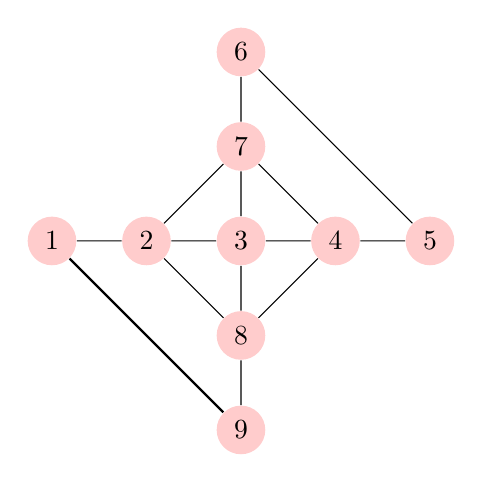
\begin{tikzpicture}
  [scale=.6,auto=left,every node/.style={circle,fill=red!20}]
  \node (n1) at (1,7) {1};
  \node (n2) at (3,7)  {2};
  \node (n3) at (5,7)  {3};
  \node (n4) at (7,7) {4};
  \node (n5) at (9,7)  {5};
  \node (n6) at (5,11)  {6};
   \node (n7) at (5,9) {7};
   \node (n8) at (5,5) {8};
   \node (n9)  at (5,3) {9};
  \foreach \from/\to in {n1/n2,n2/n3,n3/n4,n4/n5,n6/n7,n7/n3,n3/n8,n8/n9,n2/n7,
  n4/n7,n4/n8,n8/n2,n6/n5}
    \draw (\from) -- (\to);
\path[thick] (n1) edge (n9);
\end{tikzpicture}
\caption{ Closed Eulerian Walk with edge (1,9) added to Figure \ref{4g2}}\label{4g255}
\end{center}
\end{figure}

Rishnak asked how will you make graph shown in Figure \ref{4g1} to have a closed Eulerian walk. Ajur now had problem. The two vertices which have odd degrees 2 and 4, have an already an edge between them. However, he remembered the definition of a multigraph, where in between any two vertices, there can be more than one edge. So he added another edge between 2 and 4 and there is a closed Eulerian walk 2-3-4-1-2-4-2. Ajur again drew a graph as shown in Figure \ref{4g155}
Ajur added that if a graph is not connected, there is neither Eulerian walk nor a closed Eulerian walk.
\begin{figure}
\begin{center}
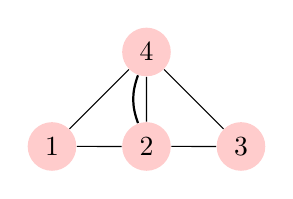
\begin{tikzpicture}
  [scale=.6,auto=left,every node/.style={circle,fill=red!20}]
  \node (n1) at (1,7) {1};
  \node (n2) at (3,7)  {2};
  \node (n3) at (5,7)  {3};
  \node (n4) at (3,9)  {4};

  \foreach \from/\to in {n1/n2,n2/n3,n2/n4,n1/n4,n3/n4}
    \draw (\from) -- (\to);
\path[thick] (n2) edge[bend left=20] (n4);
\end{tikzpicture}
\caption{ Graph in Figure \ref{4g1} with edge (2,4) added to have a closed Eulerian Walk}\label{4g155}
\end{center}
\end{figure}

\vspace{3in}
Rishnak asked Ajur whether he knew about multi graphs and directed graphs. Ajur realized he essentially learnt about multigraphs  by doing Eulerian walks and completion  example. Ajur added that in a direct an edge $(x,y)$ goes from vertex $x$ to $y$ and he drew an example graph to show Rishnak that he knows See Figure \ref{4g5}. Ajur mentioned that instead of degree of a vertex, we have in-degree and out-degree of a vertex. The number of edges coming to a vertex is the in-degree of that vertex and the number of edges going out of a vertex is the out-degree of a vertex. For example, in the directed graph shown in Figure \ref{4g5}, vertex 1 has in-degree 2 and out-degree 1, Each of Vertex 3 and 4 has in-degree  and out-degree 1. A directed graph is strongly connected if there is a directed path from every vertex to every other vertex. For example, directed graph shown in Figure \ref{4g5} is strongly connected. 
\begin{figure}
\begin{center}
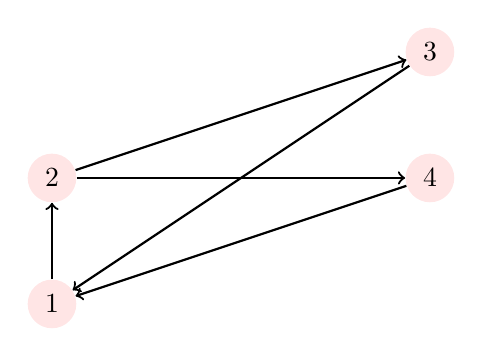
\begin{tikzpicture}
  [scale=.8,auto=left,every node/.style={circle,fill=red!10}]
  \node (n1) at (1,7) {1};
  \node (n2) at (1,9)  {2};
  \node (n3) at (7,11)  {3};
  \node (n4) at (7,9) {4};
 \path[->, draw,thick] 
        (n1) edge (n2)
         (n3) edge (n1)
        (n2) edge (n3)
        (n2) edge (n4)
        (n4) edge  (n1);

\end{tikzpicture}
\caption{ Example Directed Graph with 4 vertices and 5 edges}\label{4g5}
\end{center}
\end{figure}

Anticipating what Rishnak is going to ask, Ajur responded by saying that there is no closed Eulerian walk in this directed graph. Rishnak reminded that he wanted whether Ajur knew an Euler walk from vertex 2 to vertex 1. Ajur reasoned in a  manner similar to what he did before. Ajur saw a directed cycle (1,(1,2),2,(2,3),3,(3,1),1) or simply (1,2,3,1). So AJur was able to write the Eulerian walk as 2-3-1-2-4-1. Ajur said to have a closed Eulerian walk, you should have a collection of edge disjoint cycles (no edge is common between these cycles). In such a case, the in-degree of each vertex should be the same as its out-degree (this is similar to the degree of every vertex has to be even number as in the case of undirected graphs). for an Eulerian walk, it has start from a vertex which one more out-degree than in-degree and end in a vertex which has one more in-degree thanout-degree (For all other vertices, in-degree should be equal to out-degree).

%\chapter{Puzzle 4}
%\chapter{Puzzle 5}
%\chapter{Puzzle 6}
%\chapter{Puzzle 7}
%\chapter{Puzzle 8}
%\chapter{Puzzle 9}
%\chapter{Puzzle 10}
%\chapter{Puzzle 11}
%\chapter{Puzzle 12}
%\chapter{Puzzle 13}
%\chapter{Puzzle 14}
%\chapter{Puzzle 15}
%\chapter{Puzzle 16}
%\chapter{Puzzle 17}
%\chapter{Puzzle 18}
%\chapter{Puzzle 19}
%\chapter{Puzzle 20}
%\chapter{Puzzle 21}
%\chapter{Puzzle 22}
%\chapter{Puzzle 23}
%\chapter{Puzzle 24}
%\chapter{Puzzle 25}



% Once upon a time\ldots This document shows how you can get ePub-like formatting in \LaTeX{} with the \verb|memoir| document class. You can't yet export directly to ePub from writeLaTeX, but you can download the source and run it through a format conversion tool, such as \verb|htlatex| to get HTML, and then go from HTML to ePub with a tool like Sigil or Calibre. See \url{http://tex.stackexchange.com/questions/16569} for more advice. And they lived happily ever after.

%\lipsum

\end{document}